\documentclass[tikz]{standalone}
\usetikzlibrary{bayesnet, arrows.meta}

\begin{document}
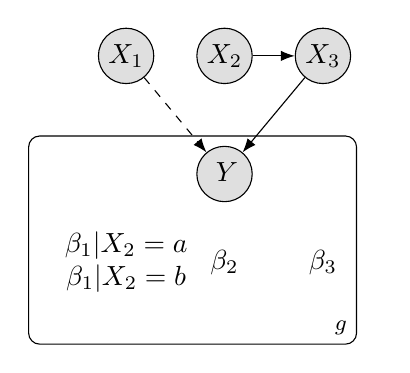
\begin{tikzpicture}


% GLOBAL SETTINGS
\newcommand{\p}{3}
\newcommand{\Xstyle}{obs}
\newcommand{\Bstyle}{}
\newcommand{\mybeta}{
\begin{tabular}{c}
\(\beta_1 | X_2 = a\) \\
\(\beta_1 | X_2 = b\)
\end{tabular}}

% SHARED CODE
\newlength{\xdist}
\setlength{\xdist}{1.25cm}
\newlength{\ydist}
\setlength{\ydist}{1.5cm}
\pgfkeys{/tikz/every path/.style={->, -{Latex[length=5pt]}}} % draw arrowheads
% X
\path (-2\xdist,\ydist) foreach \j in {1,...,\p} {
++(\xdist,0) node[\Xstyle] (X\j) {\(X_\j\)}
+(0,-1.75\ydist) coordinate (b\j) 
};
% beta
\path (-2\xdist,\ydist) foreach \j in {2,...,\p} {
(b\j) node[\Bstyle] (B\j) {\(\beta_{\j }\)}
};
\node[\Bstyle] (B1) at (b1) {\mybeta};
% helper coordinates
\path
(b1) +(-0.6\xdist,-0.0\ydist) coordinate (bL)
(b\p) +(+0.6\xdist,-0.0\ydist) coordinate (bR) ;
% Y
\node[obs] (Y) at (0,0) {\(Y_{}\)};



% EDGES & PLATE
\draw (X2) -- (X3) ;
\draw (X3) -- (Y) ;
\draw[dashed] (X1) -- (Y) ;
\plate {v-plate} {(Y) (B1) (B\p)} {\(g\)};

\end{tikzpicture}
\end{document}
